\documentclass[a4paper]{article}

\usepackage{graphicx}
\usepackage{subfig}
\usepackage{multirow}
\usepackage[utf8]{inputenc}

\graphicspath{{figuras/}}

\hyphenation{ve-ri-fi-car FalaBrasil}

\title{Relatório 01}

\author{Pedro Batista (08080002701) - pedro@ufpa.br}

\begin{document}

\maketitle

\section{Sistemas de Primeira Ordem}
   Os gráficos obtidos na experiencia são mostrados na Figura~\ref{fig:primeira_ordem},
e os valores obtidos são apresentados na Tabela~\ref{tab:primeira_ordem}.

   Pode-se observar que quando $k$ permanece constante o valor de regime também é uma constante.
E que o tempo de estabilização varia de forma aproximadamente linear com o valor de $\tau$, 
isto é, quanto maior o valor de $\tau$ mais o sistema demora para estabilizar.

   Para $\tau$ constante o tempo de estabilização também é constante. E o valor
é diretamente proporcional a $k$. Observa-se ao variar o $k$ o tempo ser
de estabilização tem que ser mesmo, caracterizando um sistema mais rápido para um
maior $k$.

\begin{figure}[h]
   \subfloat[$k=2$, $\tau =0.1$]{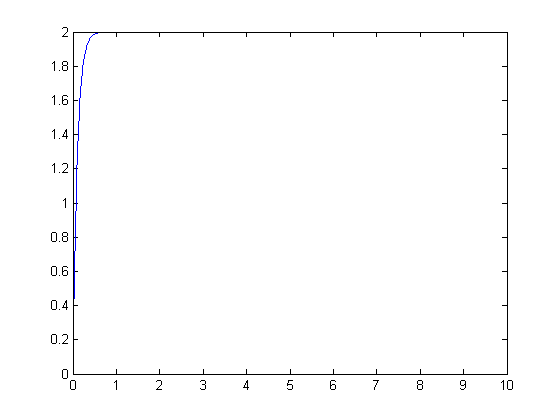
\includegraphics[width=0.5\textwidth]{k-2-tau-dot1.png}}
   \subfloat[$k=2$, $\tau =1$]{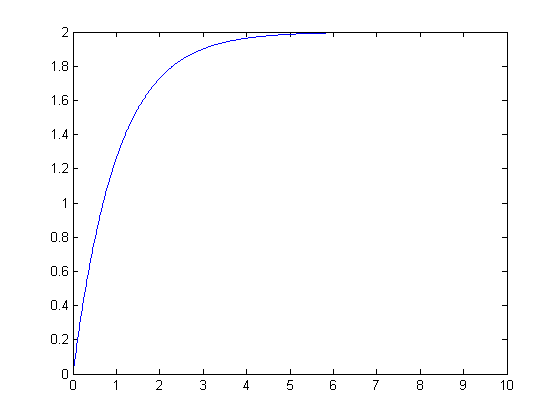
\includegraphics[width=0.5\textwidth]{k-2-tau-1.png}}\\
   \subfloat[$k=2$, $\tau =10$]{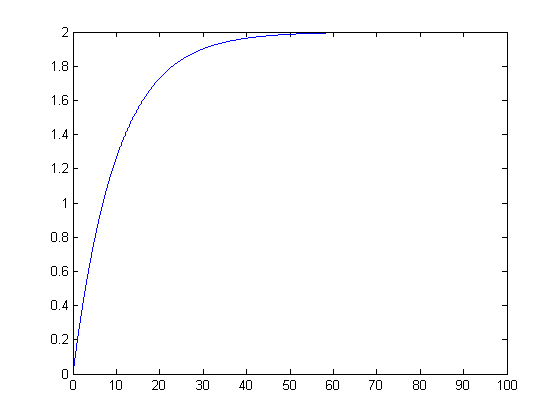
\includegraphics[width=0.5\textwidth]{k-2-tau-10.png}}
   \subfloat[$k=0.1$, $\tau =1$]{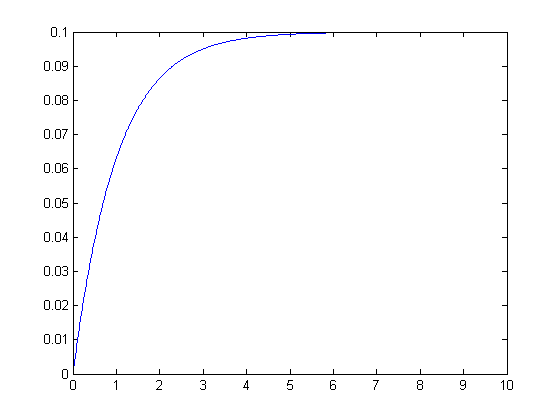
\includegraphics[width=0.5\textwidth]{k-dot1-tau-1.png}}\\
   \subfloat[$k=1$, $\tau =1$]{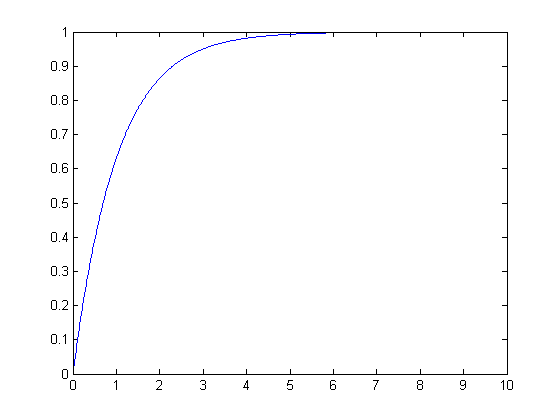
\includegraphics[width=0.5\textwidth]{k-1-tau-1.png}}
   \subfloat[$k=10$, $\tau =1$]{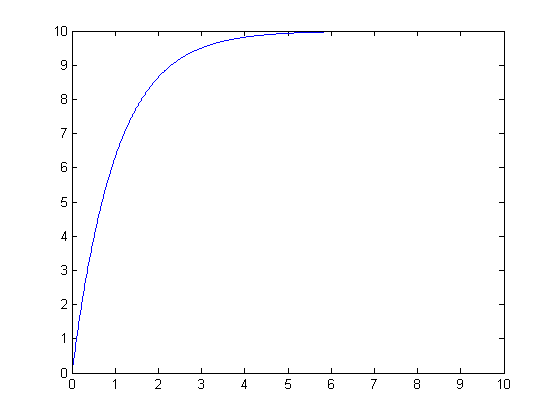
\includegraphics[width=0.5\textwidth]{k-10-tau-1.png}}
   \caption{Gráficos para sistemas de primeira ordem.}
   \label{fig:primeira_ordem}
\end{figure}

\begin{table}[h]
   \begin{center}
   \begin{tabular}{| c | c | c | c |}
      \hline
      \textbf{$k$} & \textbf{$\tau$} & \textbf{$V_r$} & \textbf{$T_e$} \\\hline
	\multirow{3}{*}{2}&	   0.1	     &	     2	      &	     0.3716    \\\cline{2-4}
	 	   &	   1	     &	     2	      &	     3.975     \\\cline{2-4}
	 	   &	   10	     &	     2	      &	     39,98     \\\hline
	 0.1	   &	   \multirow{3}{*}{1}	     &	   0.1	      &	     4.55     \\\cline{3-4} \cline{1-1}
	 1	   &	   	     &	   1	      &	     4.55     \\\cline{3-4} \cline{1-1}
	 10	   &	   	     &	   10	      &	     4.55     \\\hline
   \end{tabular}                                    
   \end{center}
   \caption{Valores medido para sistema de primeira ordem.}
   \label{tab:primeira_ordem}
\end{table}

\section{Sistemas de Segunda Ordem}

Para o sistema de segunda ordem são mostrados os gráficos na Figura~\ref{fig:segunda_ordem} e 
valores obtidos na Tabela~\ref{tab:segunda_ordem}.

Observa-se que para um melhor $\xi$ menor o sistema se torna menos estável durante sua
reposta transitória. E que para um maior $w_n$ o sistema se torna mais rápido.

\begin{figure}[h]
   \subfloat[$k=2$, $\tau =8$, $\xi = 1$]{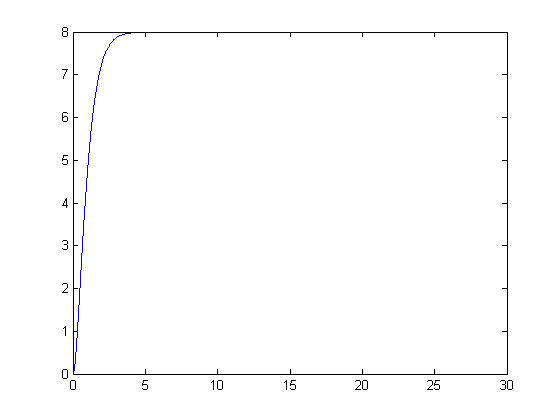
\includegraphics[width=0.5\textwidth]{wn-2-k-8-q-1.png}}
   \subfloat[$k=2$, $\tau =8$, $\xi = 0.7$]{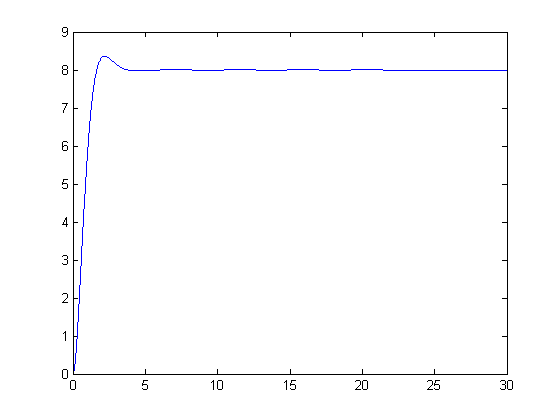
\includegraphics[width=0.5\textwidth]{wn-2-k-8-q-dot7.png}}\\
   \subfloat[$k=2$, $\tau =8$, $\xi = 0.2$]{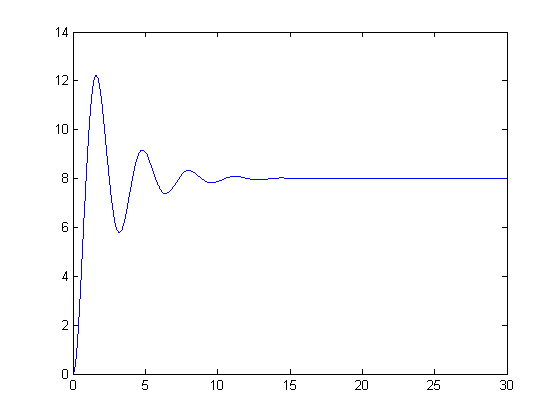
\includegraphics[width=0.5\textwidth]{wn-2-k-8-q-dot2.png}}
   \subfloat[$k=10$, $\tau =8$, $\xi = 1$]{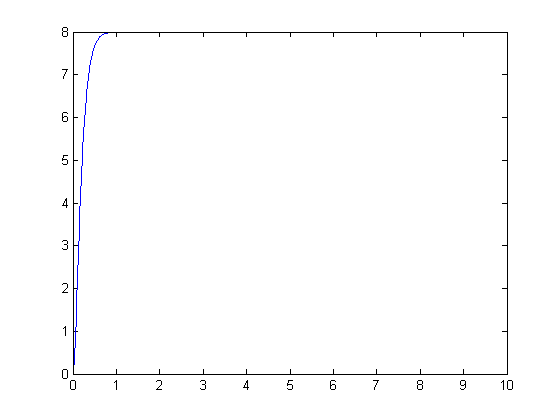
\includegraphics[width=0.5\textwidth]{wn-10-k-8-q-1.png}}\\
   \subfloat[$k=10$, $\tau =8$, $\xi = 0.7$]{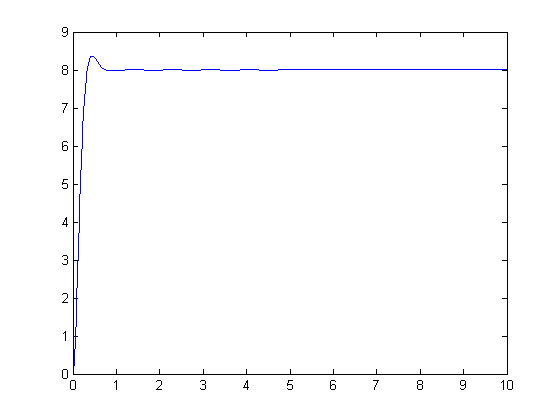
\includegraphics[width=0.5\textwidth]{wn-10-k-8-q-dot7.png}}
   \subfloat[$k=10$, $\tau =8$, $\xi = 0.2$]{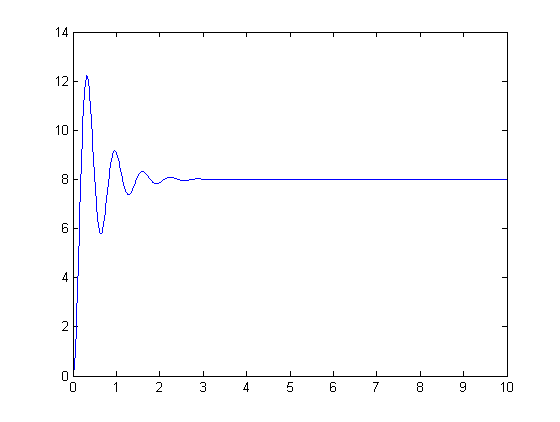
\includegraphics[width=0.5\textwidth]{wn-10-k-8-q-dot2.png}}
   \caption{Gráficos para sistemas de segunda ordem.}
   \label{fig:segunda_ordem}
\end{figure}

\begin{table}[h]
   \begin{center}
   \begin{tabular}{| c | c | c | c | c |}
      \hline
      \textbf{$w_n$} & \textbf{$k$}	      & \textbf{$\xi$} & \textbf{$T_e$} & \textbf{$M_p$} \\\hline
	\multirow{3}{*}{2} &\multirow{6}{*}{8}&	     1	      &	     2.889    &		0	 \\\cline{3-5}
	 	 	   &	   	     &	     0.7       &     2.99     &		0.368	 \\\cline{3-5}
	        	   &	   	     &	     0.2       &     9,8     &	        4.21 \\\cline{1-1} \cline{3-5}
	\multirow{3}{*}{10} &		     &	     1	      &	     0.58    &		0	 \\\cline{3-5}
	 	 	   &	   	     &	     0.7       &     0.6     &		0.368	 \\\cline{3-5}
	        	   &	   	     &	     0.2       &     0     &	        4.21 \\\hline
   \end{tabular}                                    
   \end{center}
   \caption{Valores medido para sistema de segunda ordem.}
   \label{tab:segunda_ordem}
\end{table}


\bibliographystyle{plain}
\bibliography{bib.bib} 
\end{document}
